\question % 2012 Exam, Q4.
Let $\theta$ be the angle between vectors $\vec{a} = \colvec{3}{1}{4}{-1}$ and $\vec{b} = \colvec{3}{-1}{2}{-2}$, as shown in Figure~\ref{fig:angle-between-two-vectors}.

\begin{figure}[h]
    \centering
    \begin{tikzpicture}
    \tkzDefPoints{0/0/O, 3/0/B}
    \tkzDefShiftPoint[O](45:4.243){A}
    \tkzDrawSegment[vector](O,A)
    \tkzDrawSegment[vector](O,B)
    \tkzLabelSegment[above left](O,A){$\vec{a}$}
    \tkzLabelSegment[below](O,B){$\vec{b}$}
    \tkzLabelAngle[pos=.5](B,O,A){$\theta$}
    \end{tikzpicture}
    \caption{Two vectors in three-dimensional space.}
    \label{fig:angle-between-two-vectors}
\end{figure}

\begin{parts}

\part
Find:

\begin{subparts}

\subpart[1]
$\abs{\vec{b}}$.

\begin{EnvFullwidth}
\begin{solutionorgrid}[1in]
We have
\[
    \abs{\vec{b}} = \sqrt{(-1)^2 + 2^2 + (-2)^2} = 3.
\]
\end{solutionorgrid}
\end{EnvFullwidth}

\subpart[1]
$\vec{a} \cdot \vec{b}$.

\begin{EnvFullwidth}
\begin{solutionorgrid}[1in]
We have
\[
    \vec{a} \cdot \vec{b} = 1 \times (-1) + 4 \times 2 + (-1) \times (-2) = 9.
\]
\end{solutionorgrid}
\end{EnvFullwidth}

\end{subparts}

\part[2]
Show clearly that $\displaystyle{\theta = \frac{\pi}{4}}$.

\begin{EnvFullwidth}
\begin{solutionorgrid}[1.5in]
We have
\begin{align*}
    \theta &= \arccos\!\pfrac{\vec{a} \cdot \vec{b}}{\abs{\vec{a}} \abs{\vec{b}}} \\
    &= \arccos\!\pfrac{9}{3\sqrt{2} \times 3} && (\textrm{by (a)}) \\
    &= \arccos\!\pfrac{1}{\sqrt{2}} \\
    &= \frac{\pi}{4}.
\end{align*}
\end{solutionorgrid}
\end{EnvFullwidth}

\part[2]
Given point $A(3, -4, 2)$, as shown in Figure~\ref{fig:angle-between-two-vectors-specific-case}, find $M$ and $N$ such that $\displaystyle{\angle{MAN} = \frac{\pi}{4}}$.

\begin{figure}[h]
    \centering
    \begin{tikzpicture}
    \tkzDefPoints{0/0/O, 3/0/B}
    \tkzDefShiftPoint[O](45:4.243){A}
    \tkzDrawSegment[semithick](O,A)
    \tkzDrawSegment[semithick](O,B)
    \tkzLabelPoint[above](A){$M$}
    \tkzLabelPoint[below right](O){$A(3, -4, 2)$}
    \tkzLabelPoint[right](B){$N$}
    \end{tikzpicture}
    \caption{Two line segments in three-dimensional space.}
    \label{fig:angle-between-two-vectors-specific-case}
\end{figure}

\begin{EnvFullwidth}
\begin{solutionorgrid}[1.5in]
Let $M(m_1, m_2, m_3)$ and $N(n_1, n_2, n_3)$. We want
\begin{align*}
    \vv{AM} &= \colvec{3}{m_1 - 3}{m_2 + 4}{m_3 - 2} & \vv{AN} &= \colvec{3}{n_1 - 3}{n_2 + 4}{n_3 - 2} \\
    &= \colvec{3}{1}{4}{-1}, & &= \colvec{3}{-1}{2}{-2}.
\end{align*}
Thus, $M(4, 0, 1)$ and $N(2, -2, 0)$.
\end{solutionorgrid}
\end{EnvFullwidth}

\end{parts}
